% This is main.tex, a sample paper demonstrating the use of the
% LLNCS macro package for Springer Computer Science proceedings;
% Version 2.20 of 2017/10/04
% 
\documentclass[runningheads]{llncs}
\usepackage[a4paper,left=3cm,right=3cm,top=4cm,bottom=4cm,bindingoffset=5mm]{geometry}
%
% ---- Packages ----
%
\usepackage{graphicx} % enhanced support for graphics
\usepackage{url} % add macros for handling URLs in text
\usepackage[nohyperlinks,nolist]{acronym} % abbreviation utilities
\usepackage{listings}
\usepackage{float}
\usepackage{tabularx}
% TODO: add more packages below if necessary
%
% ---- Acronyms ----
%
\begin{acronym}
\acro{rq}[RQ]{Research Question}
% TODO: define more acronyms here
\acro{llm}[LLM]{large language model}
\acro{lm}[LM]{language model}
\acro{sast}[SAST]{static application security testing}
\acro{ci}[CI]{continuous integration}
\acro{fn}[FN]{false negative}
\acro{fp}[FP]{false positive}
\acro{oss}[OSS]{open-source software}
\acro{rag}[RAG]{retrieval augmented generation}
\acro{cve}[CVE]{Common Vulnerabilities and Exposures}
\acro{bic}[BIC]{bug-inducing commit}
\acro{bfc}[BFC]{bug-fixing commit}
\end{acronym}
%
% ---- Begin Document ----
%
\begin{document}
%
\title{LLM-Augmented Static Analysis Security Testing}
%
%\titlerunning{Abbreviated paper title}
% If the paper title is too long for the running head, you can set
% an abbreviated paper title here
%
% ---- Author Information ----
%
\author{Murilo Escher Pagotto Ronchi}
\institute{Seminar: Software Quality\\
Advisor: Kohei Dozono\\
Technical University of Munich\\
\email{murilo.escher@tum.de}}
%
\maketitle % typeset the header of the contribution
%
% ---- Abstract ----
%
\begin{abstract}
Static Application Security Testing (SAST) tools are widely used to detect vulnerabilities in software systems by analyzing source code, bytecode, or binaries. However, these tools often face limitations, including false positives and difficulties in analyzing vulnerabilities caused by runtime behavior. Recent advancements in large language models (LLMs) have demonstrated their potential to enhance software security analysis, particularly when combined with traditional SAST tools.

This paper explores the integration of SAST tools with LLMs to address these limitations. By leveraging the BugOSS dataset—a collection of open-source projects with documented vulnerabilities—this study employs CodeQL and Infer to analyze vulnerabilities and gathers additional context through call graph analysis. The contextual data, including caller and callee relationships, is combined with SAST output and formatted into structured prompts for GPT-4. This approach aims to reduce false positives and improve the reasoning behind vulnerability detection.

The results reveal that while LLMs excel in reasoning about simpler vulnerabilities like null pointer dereferences, their performance diminishes for more complex issues requiring deeper code comprehension. While contextual information provided valuable insights into the code structure, its overall impact on reducing false positives was limited, as many flagged vulnerabilities were isolated or lacked meaningful interdependencies in the call graph. These findings highlight both the potential and the limitations of LLM-augmented static analysis, laying the groundwork for future research on integrating richer program representations with LLMs for enhanced security testing.

\keywords{Security testing  \and Static analysis \and Large language models.}
\end{abstract}
%
% ---- Text Parts ----
%
\section{Introduction}
\label{sec:intro}
\acp{llm} have recently gained a lot of popularity.
Among their many uses, one currently much researched possibility is their application in \ac{sast}.

Talk about repo-level being more important, \cite{risse2024scorewrongexambenchmarking} 

In this paper, we further investigate their usability when combined with \ac{sast} Tools.
\section{Related Work}
\label{sec:relwork}
Here it should be made clear how this project differs from related work.
The ways in which we improved or completed other research should be made clearer.
\newpage
\section{Methodology}
\label{sec:methodology}
This study investigates the potential of combining static analysis tools with \aclp{llm} to enhance the detection of software vulnerabilities while addressing the issue of false positives. 
The methodology involves using two static analyzers, CodeQL and Infer, to flag vulnerabilities, enriching their output with additional code context obtained through a code graph of the project, and leveraging an \ac{llm} to refine the results. 
Figure~\ref{workflow} provides an overview of the workflow.

\begin{figure}[H]
    \centering
    \resizebox{\textwidth}{!}{%
        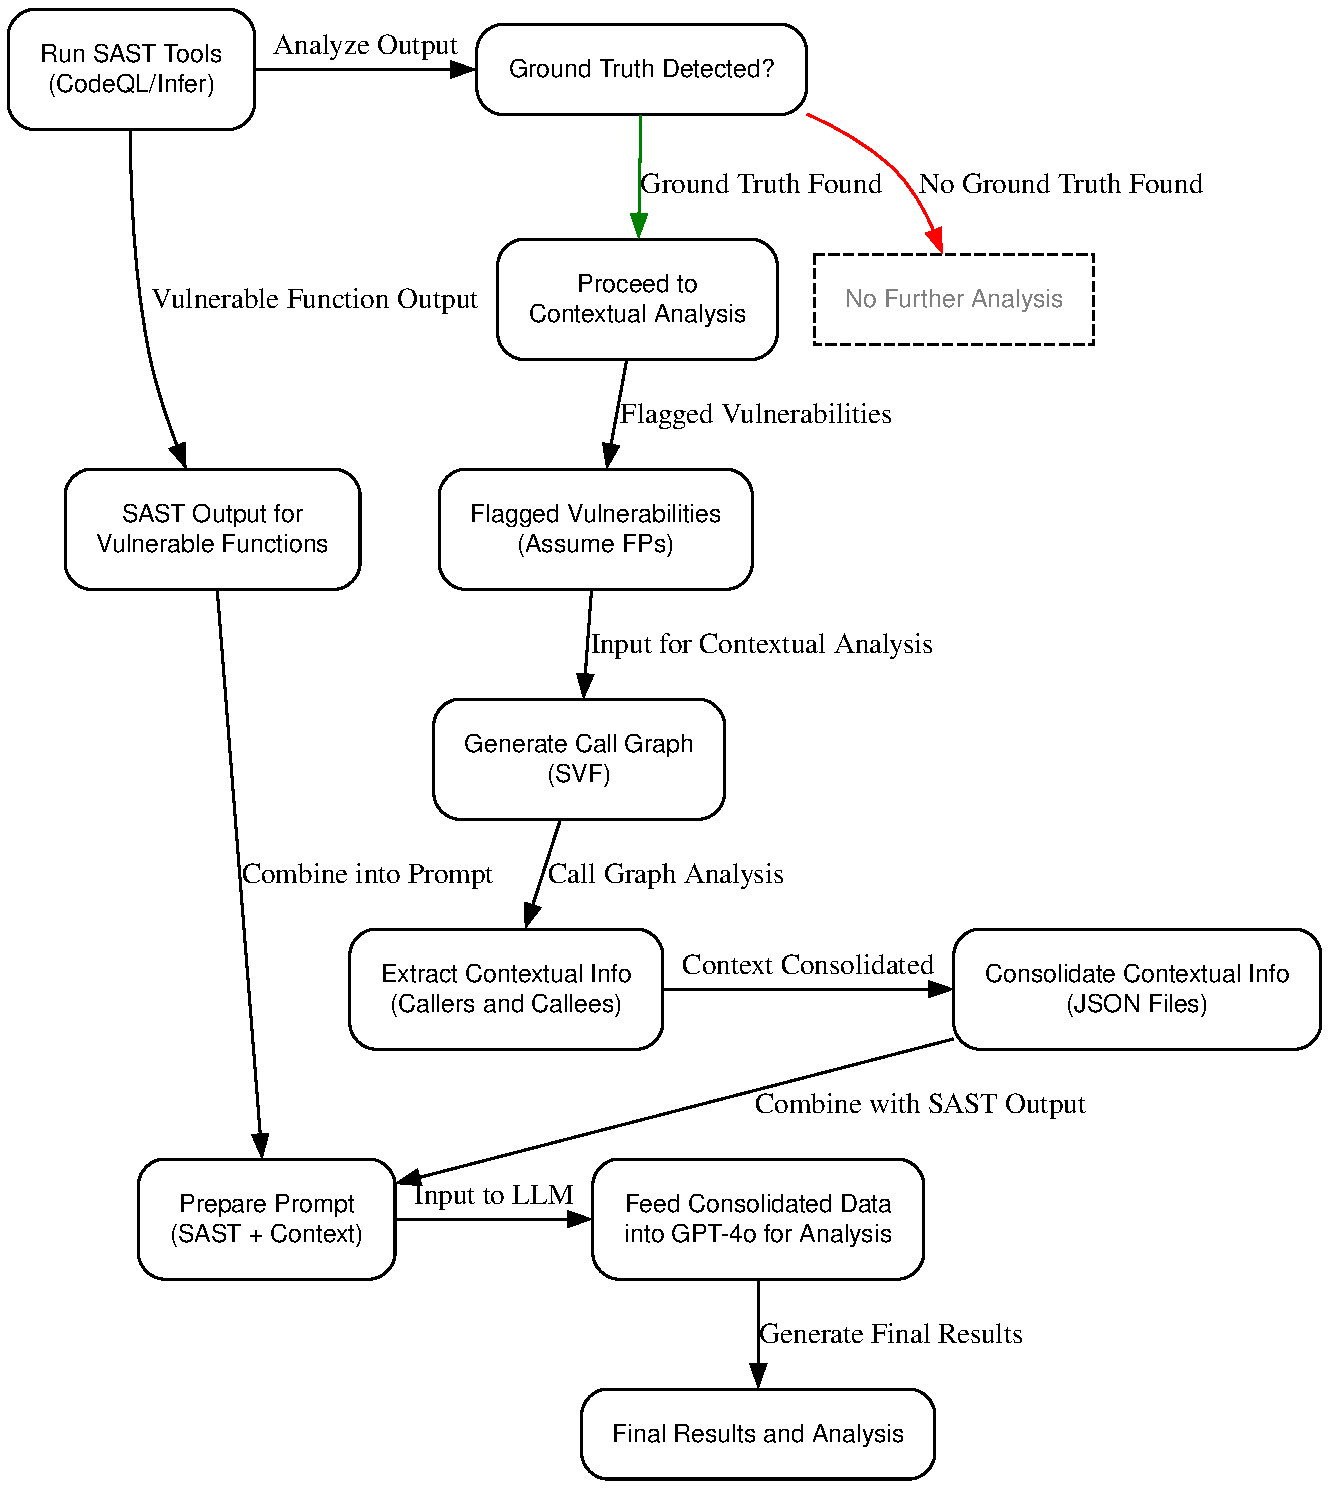
\includegraphics{figures/workflow.pdf} % Path to your diagram file
    }
    \caption{Overview of the workflow combining SAST tools, contextual analysis, and LLM augmentation.}
    \label{workflow}
\end{figure}


In each of the following subsections, detailed explanations of the tools used will be provided, with the goal of clarifying the diagram illustrated above step by step.

\subsection{Dataset and Ground Truths}
\label{sec:methodology:sub:dataset}
BugOSS~\cite{BugOSS} is a dataset containing vulnerabilities manually detected in various \acl{oss} projects.
It comprises a total of 21 different real-world projects, ranging from lesser known projects like Poppler~\cite{poppler}, a library used for rendering PDFs, to widely used software tools, such as Curl~\cite{curl}, a command-line tool that enables data transfer with URLs.

Despite being originally crafted for examinations through fuzz testing, BugOSS contains, for each of the listed projects, information regarding the \ac{bic}, as well as the \ac{bfc}. 
Together with corresponding Dockerfiles and build scripts for each one of the projects, this dataset proves very useful for the reproducibility of the detected vulnerabilities.
Listing~\ref{bugoss} provides a clear overview of how information is structured in the dataset.

\begin{lstlisting}[caption={Hierarchy of the BugOSS dataset}, label={bugoss}]
BugOSS Dataset
+-- Projects (21 Total)
|   \-- Project A (e.g., Poppler)
|   |   +-- Bug-Inducing Commit (BIC)
|   |   +-- Bug-Fixing Commit (BFC)
|   |   +-- Information about Failure Type
|   |   +-- Dockerfile
|   |   +-- Build Script
|   |   \-- Supporting Artifacts
|   \-- Project B (e.g., Curl)
|   |   +-- Bug-Inducing Commit (BIC)
|   |   +-- Bug-Fixing Commit (BFC)
|   |   +-- Information about Failure Type
|   |   +-- Dockerfile
|   |   +-- Build Script
|   |   \-- Supporting Artifacts
\-- Fuzz Testing Metadata
\end{lstlisting}

For this study, the selection and treatment of ground truths followed a systematic process:
\begin{enumerate}
    \item \textbf{Selection Criteria:} Out of the 21 projects in the dataset, only those that could be successfully built and reproduced using the provided Dockerfiles and build scripts were included in the analysis. While the dataset aims to ensure reproducibility, certain projects encountered build errors due to syntax errors in the code or the \ac{bic} not being in a branch. The build process consisted of reverting the repository to the \ac{bic} and using the appropriate build script. Ultimately, 19 projects were successfully built and used as the basis for further analysis.

    \item \textbf{Use of Ground Truths:} The validated vulnerabilities served as the baseline for evaluating the performance of static analysis tools. For each successfully built project, the outputs of the tools were analyzed to determine whether they could detect the known vulnerabilities. The ground truth was considered to be found if the static analyzer flagged a vulnerability in the function containing it, even if not in the same line.
\end{enumerate}

It is also worthy to mention that the provided Dockerfiles and build scripts needed to be slightly modified. For the Dockerfiles it was necessary to add commands so that both static analyzers were installed during the image creation, and the build scripts needed to be adapted so that the last build command was not directly executed, but instead passed to the corresponding tool, according to their documentation. 

\subsection{Static Analysis with CodeQL and Infer}
\label{sec:methodology:sub:sast}
To evaluate the potential of static analysis tools in detecting vulnerabilities, this study utilized two widely known tools: CodeQL and Infer. These tools were selected for their distinct methodologies—CodeQL's query-based analysis and Infer's focus on memory-related issues—and their relevance in the field of software security. Together, they represent complementary approaches to vulnerability detection in real-world software projects.

\subsubsection{CodeQL}
Developed by GitHub, CodeQL is a query-based static analysis tool that generates a database representation of a codebase, enabling developers to query their code as though it were a database. CodeQL excels at identifying vulnerabilities such as:
\begin{itemize}
    \item SQL injection,
    \item Cross-site scripting (XSS), and
    \item Insecure deserialization.
\end{itemize}

For this study, the standard library of 60 predefined queries provided by CodeQL's base installation was used without customization. While highly effective for analyzing web applications and languages like JavaScript and Python, CodeQL's performance in detecting vulnerabilities in C/C++ codebases was limited. This analysis found that CodeQL struggled to detect vulnerabilities relevant to C/C++ projects, such as memory-related issues, and often produced very few or no results for the BugOSS projects.

To run CodeQL, the provided build scripts from the BugOSS dataset were adapted to work with CodeQL's database creation process. Instead of running the \texttt{make} command (or its corresponding equivalent depending on the build setup) directly, the build command was passed to CodeQL's CLI, which intercepted the build process and generated the required database for analysis.

\subsubsection{Infer}
Developed by Meta, Infer is a static analysis tool designed to identify specific classes of vulnerabilities commonly found in C and C++ codebases. Its strengths include detecting:
\begin{itemize}
    \item Null pointer dereferences,
    \item Memory leaks, and
    \item Thread safety violations.
\end{itemize}

Infer uses symbolic execution to analyze paths through the program's control flow, identifying potential bugs. Due to its specialization in memory-related bugs, Infer proved highly effective for analyzing the C/C++ projects in the BugOSS dataset. However, limitations in build system support were observed: the Harfbuzz project could not be analyzed because its Ninja build system is not supported by Infer. This highlights a key challenge when dealing with non-standard or less commonly supported build configurations.

Similar to CodeQL, Infer required modifications to the BugOSS build scripts. Instead of executing the build command directly, the command was passed through Infer's CLI, allowing it to hook into the build process and analyze the code during compilation.

\subsubsection{Comparison and Application in This Study}
Both tools were run on the successfully built projects from the BugOSS dataset. The application process differed:
\begin{itemize}
    \item \textbf{CodeQL}: Required the creation of a database for each project using its build process.
    \item \textbf{Infer}: Analyzed the source code directly without requiring additional preprocessing.
\end{itemize}

The effectiveness of each tool was heavily influenced by the types of vulnerabilities they were designed to detect. Given that the BugOSS dataset consists largely of C/C++ projects:
\begin{itemize}
    \item \textbf{Infer's specialization in memory-related issues} resulted in a significantly higher number of detected vulnerabilities across all projects.
    \item \textbf{CodeQL's default query set} was not well-suited for C/C++ projects and detected very few or no bugs in many cases.
\end{itemize}

This stark difference highlights the importance of tool selection and configuration in vulnerability analysis, especially when analyzing language-specific codebases. The results underline the need to consider the characteristics of the codebase and vulnerabilities when choosing and setting up static analysis tools.

Given that only one ground truth vulnerability was detected across all analyzed projects - specifically, in the PcapPlusPlus project using Infer - this study followed through with PcapPlusPlus for deeper contextual analysis. In addition to the ground truth vulnerability, flagged vulnerabilities detected by Infer in PcapPlusPlus, which were assumed to include false positives, were also analyzed further. The project thus provided a suitable basis for evaluating both the limitations of static analysis tools and the potential to gather contextual information for reducing false positives among flagged vulnerabilities.


\subsection{Contextual Analysis with SVF}
\label{sec:methodology:sub:context}
To gather contextual information about the flagged vulnerable functions, the chosen method was to identify which other functions were their callers and callees. This required generating and analyzing the call graph of the code. A call graph is a representation of a program in the form of a control-flow graph. In this structure:
\begin{itemize}
    \item Each function is depicted as a node.
    \item The relationships between functions, such as function calls, are represented as edges connecting the nodes.
\end{itemize}

This representation reveals how vulnerable functions interact with other parts of the code, facilitating the extraction of contextual information.

For this analysis, the focus was on the PcapPlusPlus project, as it was the only project for which a ground truth vulnerability was detected by a static analysis tool (Infer). To generate the call graph, the \textbf{Static Value-Flow Analysis Framework for Source Code (SVF)}~\cite{svf} was used. SVF is a code analysis tool that enables interprocedural dependence analysis for LLVM-based languages. By providing SVF with a bytecode file generated using the \textbf{LLVM compiler}, the framework produces a .dot file that describes the call graph.

\textbf{LLVM} is an open-source compiler framework widely used for program analysis. It compiles source code into an intermediate representation called LLVM bytecode, which can then be analyzed by tools like SVF. The \texttt{.dot} file generated by SVF serves as a textual representation of the call graph. Figure~\ref{callgraph} illustrates how the \texttt{.dot} formatting translates into a visual representation of a call graph, with nodes representing functions and edges representing calls between them.

\begin{figure}[ht]
    \centering
    \begin{minipage}[t]{0.45\textwidth}
        \vspace{0pt} % Ensure no offset at the start of the minipage
        \begin{lstlisting}
digraph G {
    a [label="Function A"];
    b [label="Function B"];
    c [label="Function C"];
    a -> b;
    a -> c;
}
        \end{lstlisting}
        \vspace{0.5em} % Space between lstlisting and custom caption
        {\footnotesize Call graph in .dot file format.} % Manually add caption text
    \end{minipage}
    \hfill
    \begin{minipage}[t]{0.45\textwidth}
        \vspace{0pt} % Ensure no offset at the start of the minipage
        \centering
        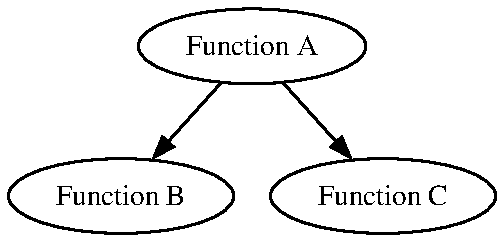
\includegraphics[width=\textwidth]{figures/callgraph.pdf}
        \vspace{0.5em} % Optional space for consistency
        {\footnotesize Graphical representation of the call graph.} % Manually add caption text
    \end{minipage}
    \caption{Comparison of the textual and graphical representation of the call graph.}
    \label{callgraph}
\end{figure}

After generating the call graph, the next step was to filter out the vulnerable functions obtained as described in Subsection~\ref{sec:approach:sub:sast}. This involved:
\begin{enumerate}
    \item Using a Python script to match the function names to the corresponding node labels in the graph. This step was necessary because the nodes in the \texttt{.dot} file are not directly named after the functions, as shown in Figure~\ref{callgraph}.
    \item Performing some manual filtering to address mismatches and inconsistencies in the node labeling.
\end{enumerate}

To navigate the graph and extract callers and callees of the vulnerable functions, the \textbf{pydot} library~\cite{pydot} was used. This Python library efficiently handled the parsing of the \texttt{.dot} file and allowed for the lookup of relevant edges and connected functions, making it easier to analyze the relationships between the nodes.

Once the relevant functions and their contexts were extracted, the results were stored in \texttt{.json} files for further analysis. These files contained details about the vulnerable functions and their relationships with other functions in the graph (e.g., callers and callees). 

Despite this focus, only 11 out of the 51 vulnerabilities detected in PcapPlusPlus appeared in the call graph generated by SVF. This discrepancy highlights a limitation in the representation or the analysis process, as certain vulnerabilities may correspond to code that was not captured or connected in the generated call graph.


\subsection{LLM Augmentation}
\label{sec:methodology:sub:llm}
To enhance the static analysis process and reduce false positives, this study utilized a Large Language Model (LLM), specifically GPT-4o, to analyze and reason about flagged vulnerabilities. The aim of this augmentation was to leverage the LLM's natural language understanding and contextual reasoning capabilities to refine the results obtained from static analysis tools.

\subsubsection{Data Consolidation and Prompt Construction}
To facilitate the analysis by GPT-4, the following information was consolidated for each flagged vulnerability:
\begin{enumerate}
    \item \textbf{Static Analysis Results}: Details from the SAST tools, including the type of vulnerability, file and line location, and any other explanatory information provided by the tool.
    \item \textbf{Contextual Information}: The callers and callees of the flagged function derived from the SVF-generated call graph, as well as the source code for the actual function.
\end{enumerate}

Given that some functions had numerous callers and callees, it was impractical to include the complete code for them directly in the prompt. Instead, the code for all relevant functions (callers, callees, and the flagged function) was extracted from the codebase and saved into separate files. These files were referenced in the prompt to provide GPT-4 with access to the full context while keeping the prompt concise. For files whose context could not be found, references to contextual information and the corresponding files were removed from the prompt.

\subsubsection{Prompt Structure}
The prompt provided followed the structure below:

\begin{lstlisting}[breaklines=true, caption={Prompt structure for GPT-4 analysis of flagged vulnerabilities.}, label={prompt}]
I want you to help me determine whether the following function is vulnerable or not.
The input consists of:
- Results from a static analysis tool, Infer.
- Contextual information in the form of callers and callees derived from a call graph.
- Files containing the full code for related functions.

Static Analysis Results:
- The full static analysis results from Infer for the flagged function are available in the following file:
    - Callers: report.json

Contextual Information:
- Code Files: The full code for the flagged function, its callers, and its callees is available in the following files:
    - Flagged Function: flagged_function.txt
    - Callers: callers.txt
    - Callees: callees.txt

Task:
Analyze the above information and determine whether the flagged vulnerability is likely a false positive. Provide your reasoning.
\end{lstlisting}

Once the prompt was constructed, it was input into GPT-4 through ChatGPT. Each prompt corresponded to a flagged vulnerability, and the LLM was tasked with:
\begin{itemize}
    \item Determining whether the vulnerability was a true positive or a false positive.
    \item Providing reasoning for the classification, referencing both the SAST output and contextual information.
\end{itemize}

By combining structured outputs from static analysis tools with external code files and contextual information, the prompts leveraged GPT-4’s ability to reason about software vulnerabilities in a way that SAST tools alone could not. This approach aimed to:
\begin{itemize}
    \item Reduce false positives by incorporating code context into the analysis.
    \item Enhance explainability by producing detailed reasoning for each classification.
\end{itemize}


\subsection{Summary}
\label{sec:methodology:sub:summary}
This section presented the methodology used to investigate the augmentation of static analysis with large language models for enhanced vulnerability detection. The process was structured into several key steps:
\begin{enumerate}
    \item Dataset Selection: The BugOSS dataset was used as the basis for this study, providing a collection of real-world projects with known vulnerabilities. The dataset enabled reproducible experiments by including bug-inducing and bug-fixing commits alongside build scripts for each project.
    \item Static Analysis: Two widely used static analysis tools, CodeQL and Infer, were employed to detect vulnerabilities. While CodeQL struggled with C/C++ projects, Infer successfully identified a ground truth vulnerability in the PcapPlusPlus project. This project was selected as the focus of the subsequent analysis.
    \item Contextual Analysis: Using SVF, a call graph of the PcapPlusPlus project was generated to extract contextual information about flagged functions. Callers and callees of these functions were identified and consolidated for deeper reasoning about the flagged vulnerabilities.
    \item LLM Augmentation: The outputs from the static analysis tools and contextual analysis were combined into structured prompts for GPT-4. By leveraging the LLM's reasoning capabilities, this step aimed to reduce false positives and enhance the interpretability of the analysis results.
\end{enumerate}

By integrating static analysis tools, contextual information, and GPT-4, this methodology proposes an approach to addressing key limitations of traditional static analysis. The next section evaluates the effectiveness of this approach in terms of its ability to detect vulnerabilities and reduce false positives.
\section{Results}
\label{sec:results}
Each of the following topics presents the results of the subsections discussed in Section~\ref{sec:methodology}.

\subsubsection{Project Builds}
As mentioned in Subsection~\ref{sec:methodology:sub:dataset}, only 19 out of the 21 projects contained in BugOSS could be successfully built. These projects were then used with the static analyzers. The fact that not all projects could be built points to a flaw in BugOSS regarding reproducibility.

\subsubsection{Static Analysis Results}
To evaluate the detection capabilities of the static analysis tools, both CodeQL and Infer were run on the 19 successfully built projects. The number of flagged vulnerabilities for each project is summarized in Table~\ref{sast_results}. It is important to denote that Infer could not be executed on Harfbuzz due to its unsupported build system.

\begin{table}[ht]
\centering
\caption{Number of vulnerabilities flagged by CodeQL and Infer for each project.}
\label{sast_results}
\begin{tabular}{|l|c|c|}
\hline
\textbf{Project Name} & \textbf{Flagged by CodeQL} & \textbf{Flagged by Infer} \\
\hline
Arrow & 0 & 71 \\
Aspell & 0 & 63 \\
Curl & 5 & 33 \\
Exiv2 & 3 & 55 \\
File & 0 & 107 \\
Gdal & 152 & 876 \\
Grok & - & - \\
Harfbuzz & 0 & - \\
Leptonica & 1 & 200 \\
Libarchive & 2 & 200 \\
Libhtp & 1 & 15 \\
Libxml2 & - & - \\
Ndpi & 5 & 75 \\
Openh264 & 11 & 191 \\
OpenSSL & 55 & 200 \\
PcapPlusPlus & 1 & 51 \\
Poppler & 15 & 200 \\
Readstat & 3 & 66 \\
Usrsctp & 2 & 0 \\
Yara & 1 & 24 \\
Zstd & 2 & 20 \\
\hline
Total & \textbf{259} & \textbf{2447} \\
\hline
\end{tabular}
\end{table}

As shown in the table, CodeQL flagged significantly fewer vulnerabilities compared to Infer. While Infer specializes in detecting memory-related vulnerabilities, CodeQL's default query set focuses on issues like SQL injection and cross-site scripting, which are uncommon in this dataset. CodeQL's analysis could possibly be improved with customized queries adapted to the nature of the projects in question.

The high amounts of flagged vulnerabilities by Infer is a great example as to why SAST tools present a challenge for a very effective and seamless continuous use. Sifting through so many warnings, searching for true positives, proves to be very strenuous and time-consuming for developers. The approach presented in this paper hopes to reduce the number of warnings which would then need to be manually checked.

\subsubsection{Gathering Contextual Information}
As previously mentioned 9, of the vulnerabilities flagged by Infer were found in the call graph and used for analysis in this step. Table~\ref{context} provides an overview of how many callers and callees each of the 9 functions had.

\begin{table}[ht]
\centering
\caption{Number of relevant callers and callees found per function analyzed.}
\label{context}
\begin{tabular}{|l|c|c|}
\hline
\textbf{Function} & \textbf{\#Callers} & \textbf{\#Callees} \\
\hline
light\_create\_default\_file\_info & 1 & 0 \\
light\_create\_file\_info & 1 & 0 \\
light\_pcapng\_open\_read & 1 & 0 \\
light\_pcapng\_open\_write & 2 & 0 \\
pcpp::IDnsResource::decodeName & 1 & 4 \\
pcpp::IDnsResource::encodeName & 2 & 4 \\
pcpp::IPFilter::convertToIPAddressWithLen & 1 & 13 \\
pcpp::IPv4Layer::parseNextLayer & 8 & 37 \\
pcpp::IPv6Layer::parseExtensions & 3 & 11 \\
\hline
\end{tabular}
\end{table}

It is important to note that function calls pertaining to the C/C++ standard libraries, the LLVM compiler or any other compilation step, like an address sanitizer, that did not correspond to a function in the PcapPlusPlus repository, were not considered in this analysis, since they went out of the scope of the project.

As explained in Subsections~\ref{sec:methodology:sub:context} and~\ref{sec:methodology:sub:llm}, the source code for all these functions was gathered in separate files, whose paths were then given in the prompt.

\subsubsection{LLM Analysis}
Figure~\ref{chart} depicts the results of the LLM analysis by showing how the 51 functions examined fared in terms of false or true positives.
Regarding these results, there are some interesting points which must be addressed:

\begin{figure}[ht]
    \centering
    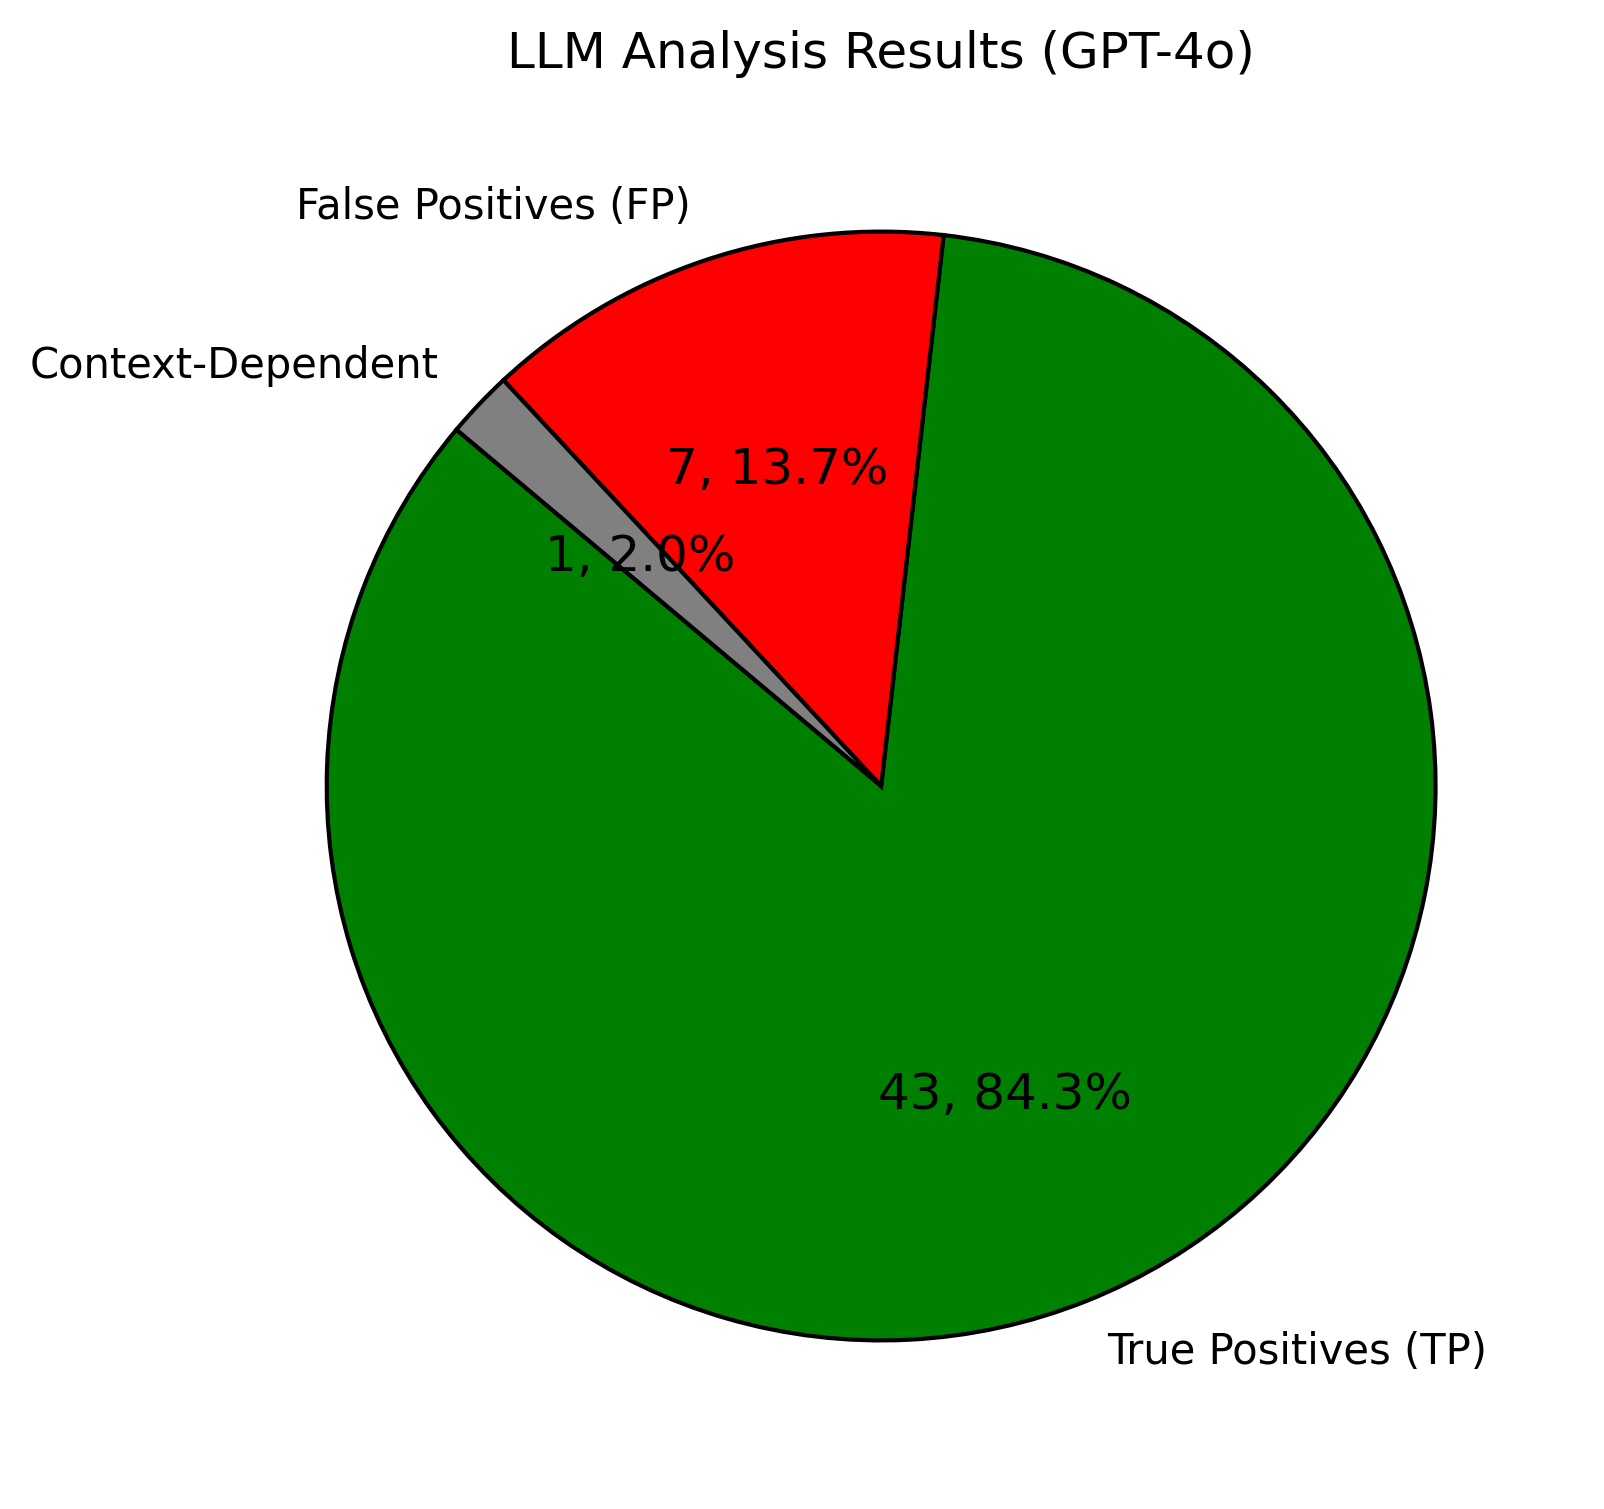
\includegraphics[scale=0.7]{figures/llm_analysis_results_with_numbers.png} 
    \caption{Results of the analysis with GPT-4o.}
    \label{chart}
\end{figure}

\begin{itemize}
    \item For one of the functions, marked in gray, the LLM did not provide a definitive answer as to whether the flagged vulnerability was a true or a false positive. Instead, it affirmed that information regarding one specific callee of the function would be necessary to come to a decision. This one callee was supposedly responsible for assigning NULL values to some fields in the data structure, which would then lead to a NULL dereference error if unchecked. Unfortunately, this callee was not picked up by SVF in the previous step, so the LLM lacked the context in this case.
    \item Many of the vulnerabilities flagged by Infer consisted in NULL dereferences, which usually appeared in the form of pointers to freshly allocated memory not being immediately checked. This type of issue is one which does not require much reasoning to correctly identify, but rather just looking for a NULL check after the allocation.
    \item Most interesting was GPT-4o's analysis of the ground truth vulnerability. As previously explained, the ground truth was considered found if the SAST tools marked any possible errors inside the same function. In the case of PcapPlusPlus, the actual problem is a buffer overflow, which happens a few lines before the dead store marked by Infer. After looking through the source code, the LLM decided that the flagged issue was a false positive, as the variable was used in pointer arithmetic. But following this verdict, it mentioned a "potential buffer issue" and pointed to the line of the ground truth, correctly explaining the reason for the vulnerability.
\end{itemize}

Table~\ref{fps} shows, for each of the 9 functions whose context could be gathered, whether GPT-4o flagged the issue as a false (FP) or true positive (TP), and the type of vulnerability originally marked by Infer. For further analysis, these functions were manually inspected to qualitatively evaluate the LLM's assessment.
\begin{table}[ht]
\centering
\caption{Qualitative Analysis from the LLM.}
\label{fps}
\begin{tabular}{|l|c|c|}
\hline
\textbf{Function} & \textbf{Verdict} & \textbf{Issue Type} \\
\hline
light\_create\_default\_file\_info & TP & NULL\_DEREFERENCE \\
light\_create\_file\_info & TP & NULL\_DEREFERENCE \\
light\_pcapng\_open\_read & TP & NULL\_DEREFERENCE \\
light\_pcapng\_open\_write & TP & NULL\_DEREFERENCE \\
pcpp::IDnsResource::decodeName & FP & DEAD\_STORE \\
pcpp::IDnsResource::encodeName & FP & DEAD\_STORE \\
pcpp::IPFilter::convertToIPAddressWithLen & TP & DEAD\_STORE \\
pcpp::IPv4Layer::parseNextLayer & TP & DEAD\_STORE \\
pcpp::IPv6Layer::parseExtensions & TP & NULL\_DEREFERENCE \\
\hline
\end{tabular}
\end{table}

As just mentioned, NULL\_DEREFERENCE issues do not require much reasoning. In the case of these functions, it was clear that there was no check after the memory allocations or function calls which changed the flagged pointers.

Regarding the DEAD\_STORE issues, there are some interesting observations, after human inspection of the warnings is done:
\begin{itemize}
    \item For decodeName, GPT-4o outputs, in its conclusion: "The flagged issue appears to be a false positive in terms of security, as decodedNameLength is not used in a way that introduces a vulnerability. However, the presence of the variable as a dead store is indicative of inefficient or unclear code, and removing or repurposing it could improve maintainability.". So, despite detecting an unused value and agreeing with the static analysis result, which is incorrect after manually analyzing the code, the model correctly phrases it as it not actually being a true positive. 
    \item In regards to encodeName, the LLM recognizes the argument flagged by Infer as a pointer which is modified, not needing to be assigned to another variable or returned for it to be considered "used".
    \item Contrary to the previous point, GPT-4o does not recognize the flagged variables in convertToIPAddressWithLen as ones modifying a memory address, which is then later used.
    \item The LLM marks the issues in parseNextLayer as true positives. However, the flagged variables are clearly used, after manual inspection, for choosing which types of layers to instantiate.
\end{itemize}

The observations above highlight the fact that there is still room for improvement regarding the model's reasoning capabilities. The outputs were correct for the most simple type of issue, the null dereference, but not for the ones which demanded greater comprehension of the code.
The LLM did, however, also show promise by correctly identifying the ground truth vulnerability, despite the issue flagged by Infer being unrelated to it.
\section{Conclusion}
\label{sec:conclusion}

You can also reference other parts of the document, e.g., sections or subsections.
In Section~\ref{sec:intro} we briefly introduced something, whereas in Subsection~\ref{sec:intro:sub:motivation}, we motivated something else.

Make sure to capitalize chapters, sections or subsections when referencing them.
\section{Threats to Validity}
\label{sec:threats}

In any empirical study, certain factors may impact the reliability and generalizability of the results. This section outlines the main limitations of the methodology.

\subsubsection{Limitations in Contextual Analysis}
The contextual analysis relied on SVF and LLVM bytecode to extract caller and callee relationships for the vulnerable functions. However, not all functions flagged by Infer were present in the call graph generated by SVF. This may indicate limitations in how SVF processes the bytecode or gaps in the way the call graph was constructed. Additionally, function names in the \texttt{.dot} file did not always match their actual representations in the source code, requiring manual mapping to align them correctly. This step introduced the possibility of errors that could impact the extracted context.

\subsubsection{Variability in LLM Responses}
LLMs such as GPT-4o are inherently non-deterministic, meaning that the same input may yield different responses across multiple runs. This poses a challenge in ensuring experimental reproducibility, as vulnerability classifications may vary if the experiment is repeated. A possible way to mitigate this issue would be to implement a voting-based approach or use multiple LLM instances to aggregate results, thereby reducing the impact of individual response variability.

\subsubsection{Manual Context Gathering}
The process of integrating static analysis results with contextual function relationships required some manual steps. Specifically, functions had to be manually filtered, formatted into structured JSON files, and cross-checked against the SVF-generated call graph. This introduces the risk of human error, which could lead to incorrect or missing contextual data. Automating these validation steps in future work would help improve reliability.

%
% ---- Appendix ----
%
\appendix
% \section{Appendix}
\label{sec:appendix}

Anything additional goes here \dots
%
% ---- Bibliography ----
%
\bibliographystyle{splncs04}
\bibliography{library.bib}
%
\end{document}